\documentclass{report}
\usepackage[margin=1.3in]{geometry}
\usepackage{amssymb}
\usepackage{amsmath}
\usepackage{syntax}
\usepackage{pdfpages}

\usepackage[T1]{fontenc}
\usepackage{lmodern}

%all used by listings
\usepackage{listings}
\usepackage{xcolor}   % for \textcolor
%\usepackage{graphicx}
\usepackage{amssymb}
\lstset{
  breaklines=true,
  frame=tblr,
  postbreak=\mbox{\textcolor{red}{$\hookrightarrow$}\space},
  basicstyle=\ttfamily\scriptsize,
  commentstyle=\color{gray}\ttfamily,
  keywordstyle=\color{blue}\ttfamily
}

\usepackage{color}
\definecolor{lightgray}{rgb}{.9,.9,.9}
\definecolor{darkgray}{rgb}{.4,.4,.4}
\definecolor{purple}{rgb}{0.65, 0.12, 0.82}
\lstdefinelanguage{TypeScript}{
  keywords={break, case, catch, class,constructor, continue, debugger, default, delete, do, else,export, false, finally, for, function, if,implements, in, instanceof, new, null, return, switch,static, this, throw, true, try, typeof, var, void, while, with},
  morecomment=[l]{//},
  morecomment=[s]{/*}{*/},
  morestring=[b]',
  morestring=[b]",
  ndkeywords={class, export, boolean, throw, implements, import, this},
  keywordstyle=\color{blue}\bfseries,
  ndkeywordstyle=\color{darkgray}\bfseries,
  identifierstyle=\color{black},
  commentstyle=\color{purple}\ttfamily,
  stringstyle=\color{red}\ttfamily,
  sensitive=true
}

%End of used by listings


\begin{document}

\chapter{Appendix}

\section{API Specification}\label{fullApiSpec}

\subsubsection{ls-projects}

\emph{Parameters}: N/A
\\
\emph{Response}: 
\begin{itemize}
\item projectnames:String[] - Returns a list of URIs for available projects on the webserver
\end{itemize} 

\subsubsection{add-project}

\emph{Parameters}: 
\begin{itemize}
\item name:String - Desired URI for the project to create
\end{itemize}
\emph{Response}: N/A

\subsubsection{get-project}
\emph{Parameters}: 
\begin{itemize}
\item project-name:String - Desired URI for the project to retrieve
\end{itemize}
\emph{Response}: 
\begin{itemize}
\item files:String[] - List of URIs for files contained within the project 
\end{itemize}

\subsubsection{add-file}
\emph{Parameters}: 
\begin{itemize}
\item project-name:String - URI for the project the file should reside in
\item file-name:String - Desired URI (relative to project) for the file to add
\end{itemize}
\emph{Response}: N/A

\subsubsection{get-file}
\emph{Parameters}: 
\begin{itemize}
\item project-name:String - URI of the project the file is in
\item file-name:String - URI (relative to project) of the file to retrieve
\end{itemize}
\emph{Response}: 
\begin{itemize}
\item ast:StructureTree - The file's "skeleton" tree consisting of nodeId's and names for these nodes to be used for navigation.
\end{itemize}

\subsubsection{save-file}
\emph{Parameters}: 
\begin{itemize}
\item project-name:String - URI of the project the file resides in
\item file-name:String - URI (relative to project) of the file to save
\end{itemize}
\emph{Response}: N/A

\subsubsection{get-node}
\emph{Parameters}: 
\begin{itemize}
\item project-name:String - URI of the project the node resides in
\item file-name:String - URI (relative to project) of the file the node resides in
\item node-id:String - The identifier of the node to retrieve
\end{itemize}
\emph{Response}: 
\begin{itemize}
\item type:String - A string describing to the client the kind of projection to be used
\item Arbitrary other attributes maybe included as required to describe the projection for this node.
\end{itemize}
\subsubsection{update-attribute}
\emph{Parameters}: 
\begin{itemize}
\item project-name:String - URI of the project the node resides in
\item file-name:String - URI (relative to project) of the file the node resides in
\item node-id:String - The identifier of the node being modified
\item attribute-name:String - The name of the attribute being modified
\item value:String - The new value of the attribute
\end{itemize}
\emph{Response}: N/A
\subsubsection{add-containment-ref}
\emph{Parameters}: 
\begin{itemize}
\item project-name:String - URI of the project the node resides in
\item file-name:String - URI (relative to project) of the file the node resides in
\item node-id:String - The identifier of the node to add the reference to
\item reference-name:String - The name of the reference feature to add a new node to
\end{itemize}
\emph{Response}: 
\begin{itemize}
\item ast:StructureTree - A tree depicting the underlying AST structure for the subtree of the node to which the child node has been added
\end{itemize}

\subsubsection{add-cross-ref}
\emph{Parameters}: 
\begin{itemize}
\item project-name:String - URI of the project the node resides in
\item file-name:String - URI of the file the node resides in
\item node-id:String - The identifier of the node to add the reference to
\item reference-name:String - The name of the reference feature to add a new node to
\item reference-file:String - The URI of the file containing the node we are referencing
\item reference-node:String - The node identifier for the node being referenced
\end{itemize}
\emph{Response}: N/A

\subsubsection{remove-ref}
\emph{Parameters}: 
\begin{itemize}
\item project-name:String - URI of the project the node resides in
\item file-name:String - URI of the file the node resides in
\item node-id:String - The identifier of the node to remove the reference from
\item reference-name:String - The name of the reference feature from which a reference will be removed
\item reference-file:String - The URI of the file containing the node we are referencing
\item reference-node:String - The node identifier for the node being referenced
\end{itemize}
\emph{Response}: N/A

\subsubsection{validate-node}

\emph{Parameters}: 
\begin{itemize}
\item project-name:String - URI of the project the node resides in
\item file-name:String - URI of the file the node resides in
\item node-id:String - The identifier of the node to validate
\end{itemize}
\emph{Response}: N/A

\section{Projection Specification Language Grammar}\label{editorLanguageGrammar}
\lstinputlisting[ tabsize=2 ]{Listings/EditorLanguage.xtext}

\section{Expression Language Definition}\label{expressionLanguageDef}
Grammar definition:
\lstinputlisting[ tabsize=2 ]{Listings/Arithmetic/Arithmetic.xtext}
Projections descriptor file:
\lstinputlisting[ tabsize=2 ]{Listings/Arithmetic/Projections.editor}

\section{Questionnaire Language Definition}\label{questionnaireLanguageDef}
Grammar definition:
\lstinputlisting[ tabsize=2 ]{Listings/Question/Q.xtext}
Projections descriptor file:
\lstinputlisting[ tabsize=2 ]{Listings/Question/Projections.editor}


\section{PasGraph Language Definition}\label{pascalLanguageDef}
Grammar definition:
\lstinputlisting[ tabsize=2 ]{Listings/Graph/Graph.xtext}
Projections descriptor file:
\lstinputlisting[ tabsize=2 ]{Listings/Graph/Projections.editor}





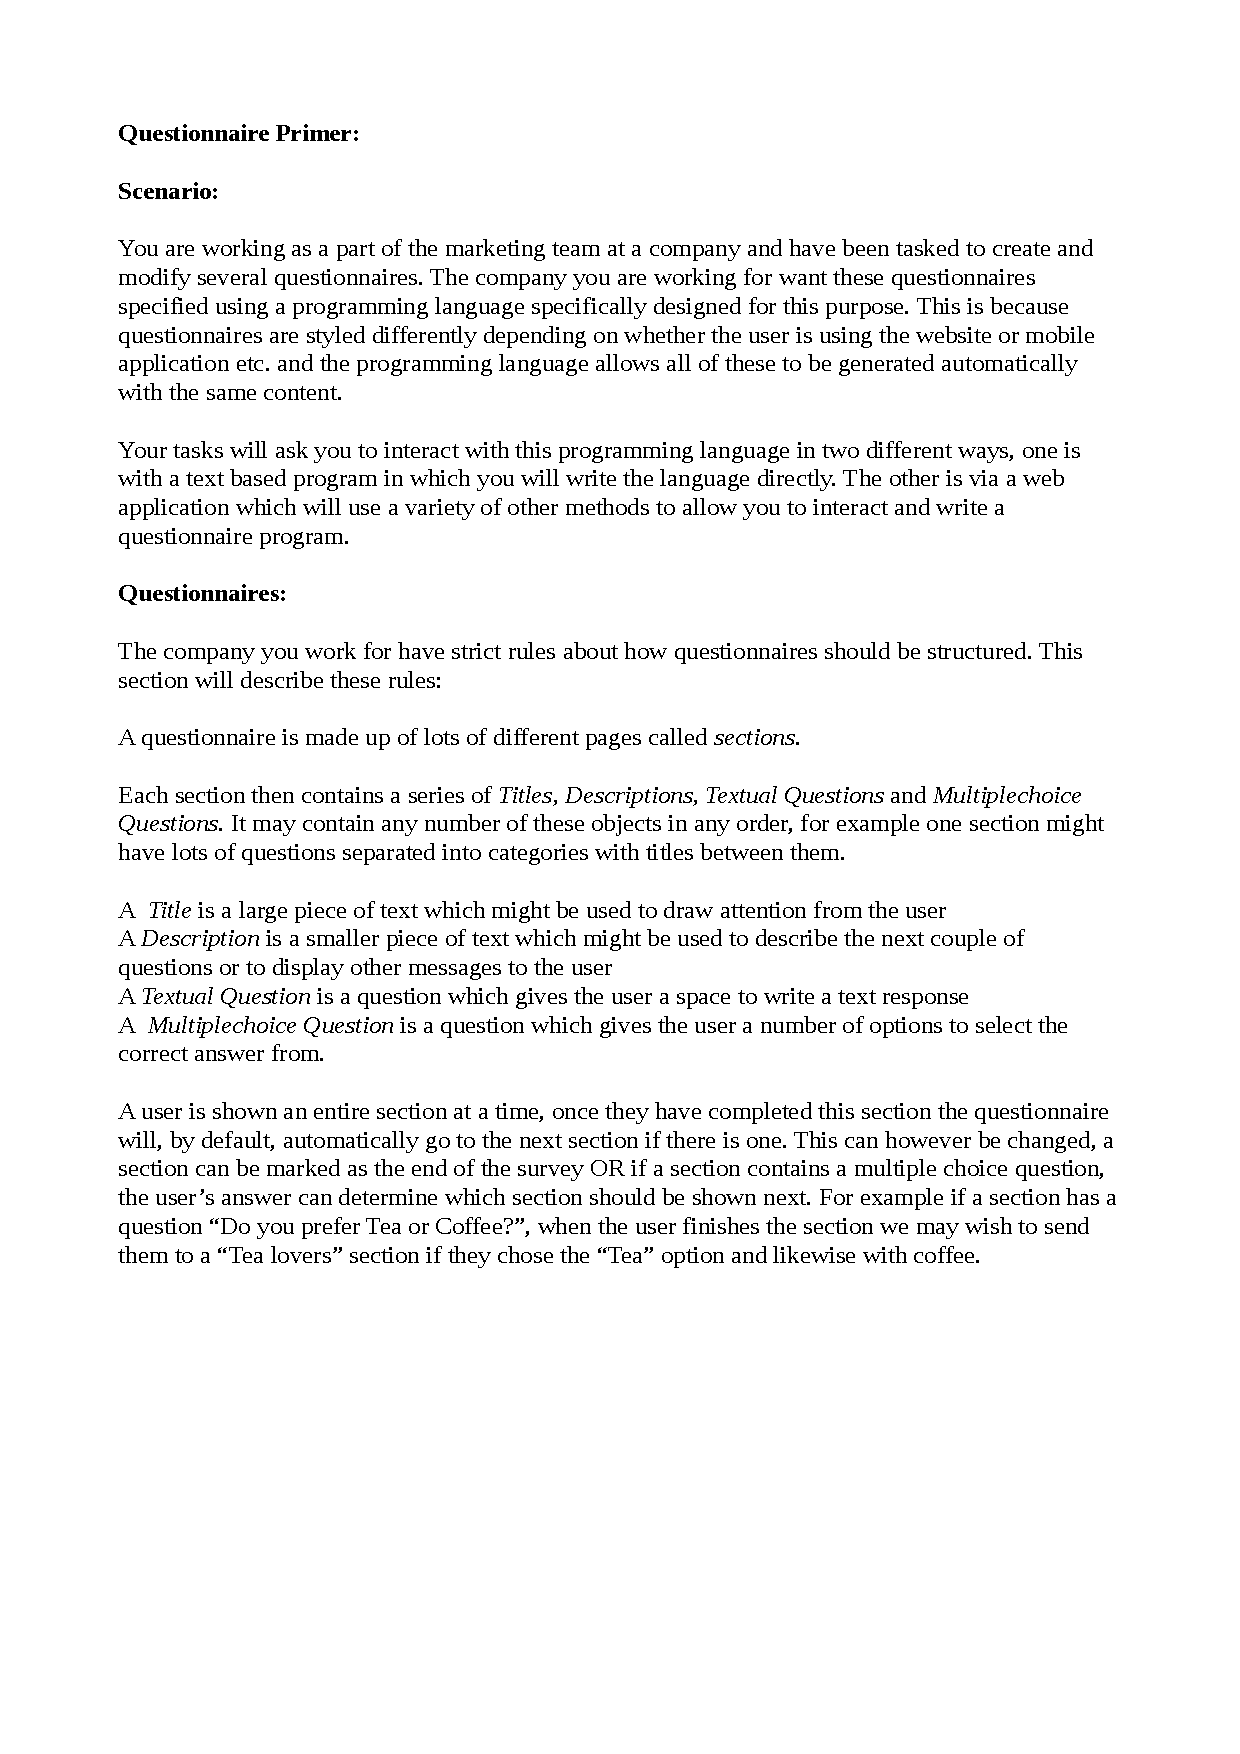
\includepdf[pages=1,scale=.75,pagecommand=\section{Questionnaire Evaluation Materials}\label{questionnaireEval} \subsection{Training Material}]{./Appendix/QuestionnaireTraining.pdf}
\includepdf[pages=2-,scale=.8]{./Appendix/QuestionnaireTraining.pdf}

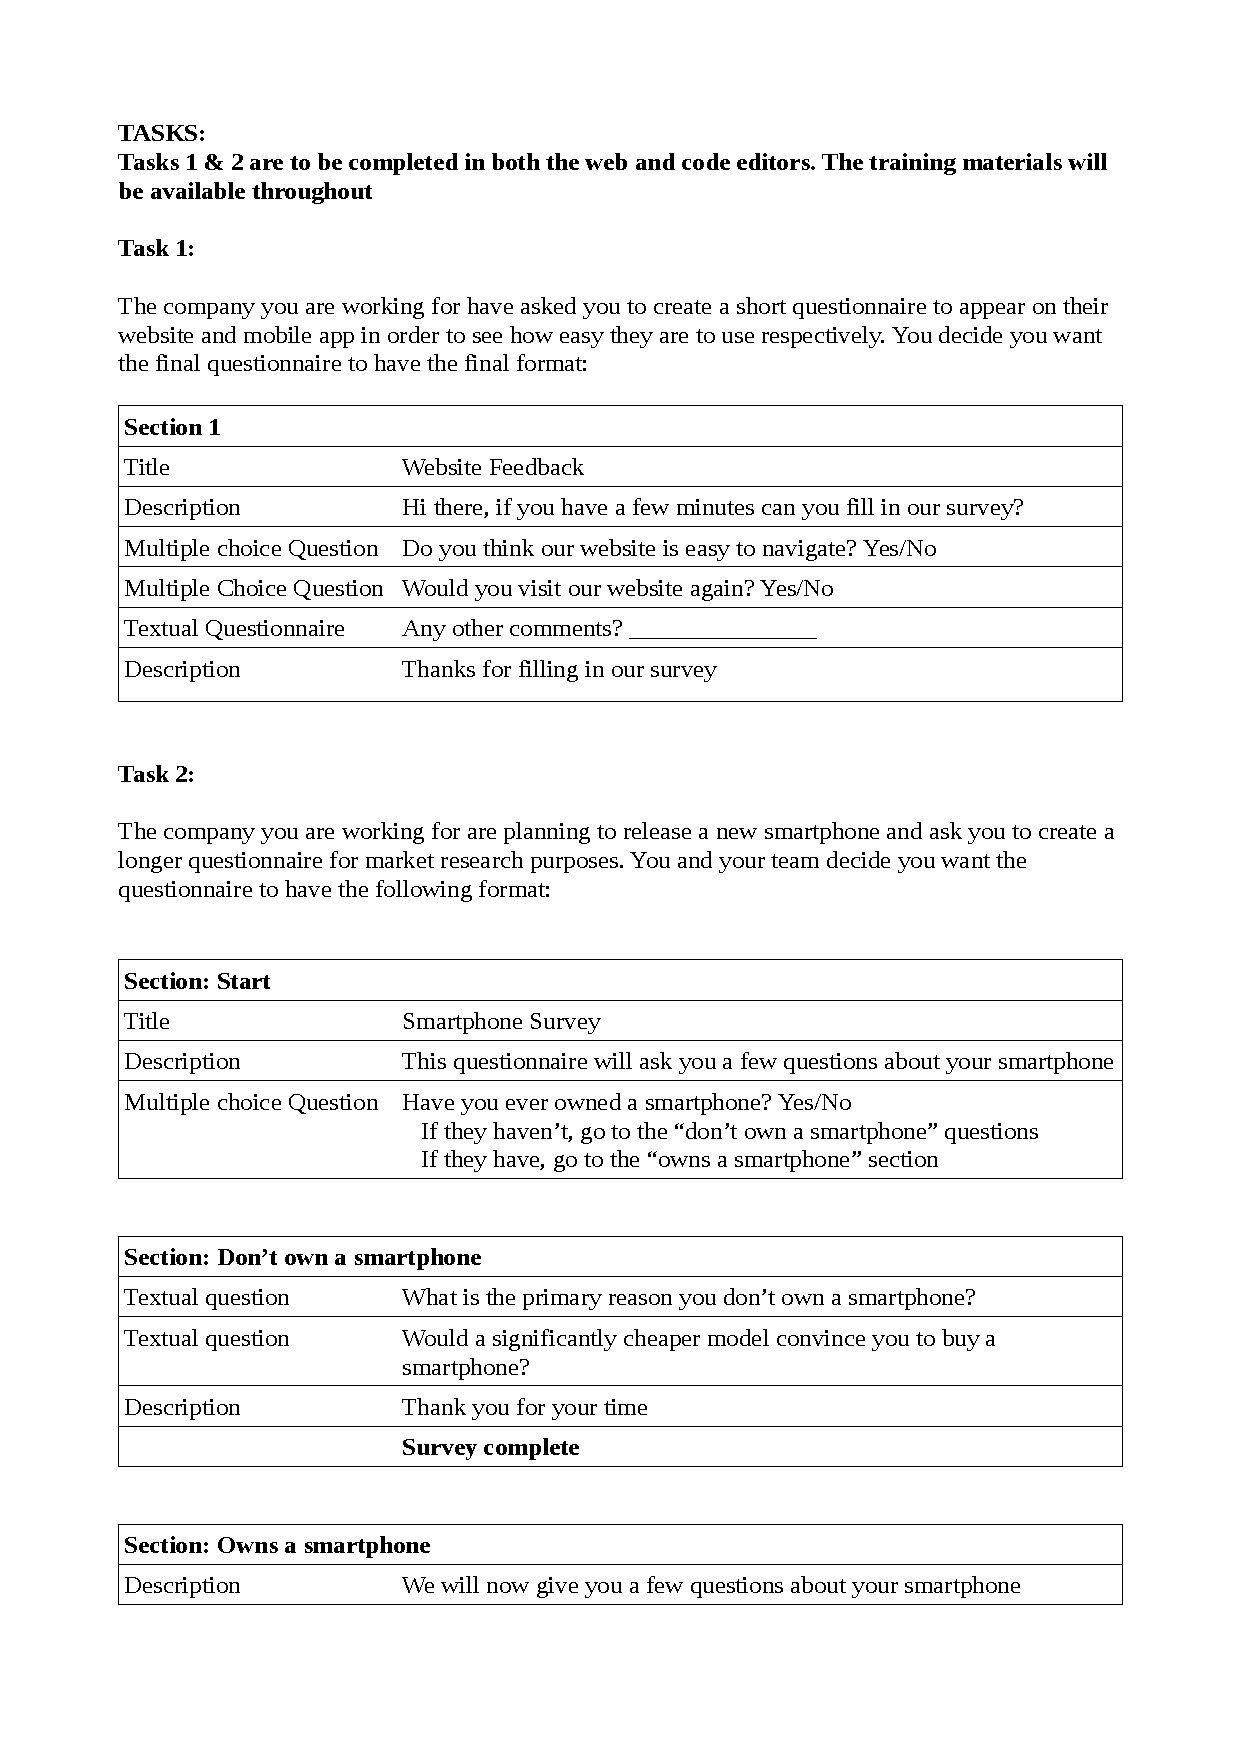
\includepdf[pages=1,scale=.8,pagecommand=\subsection{Task Sheet}]{./Appendix/QuestionnaireTasks.pdf}
\includepdf[pages=2-,scale=.8]{./Appendix/QuestionnaireTasks.pdf}

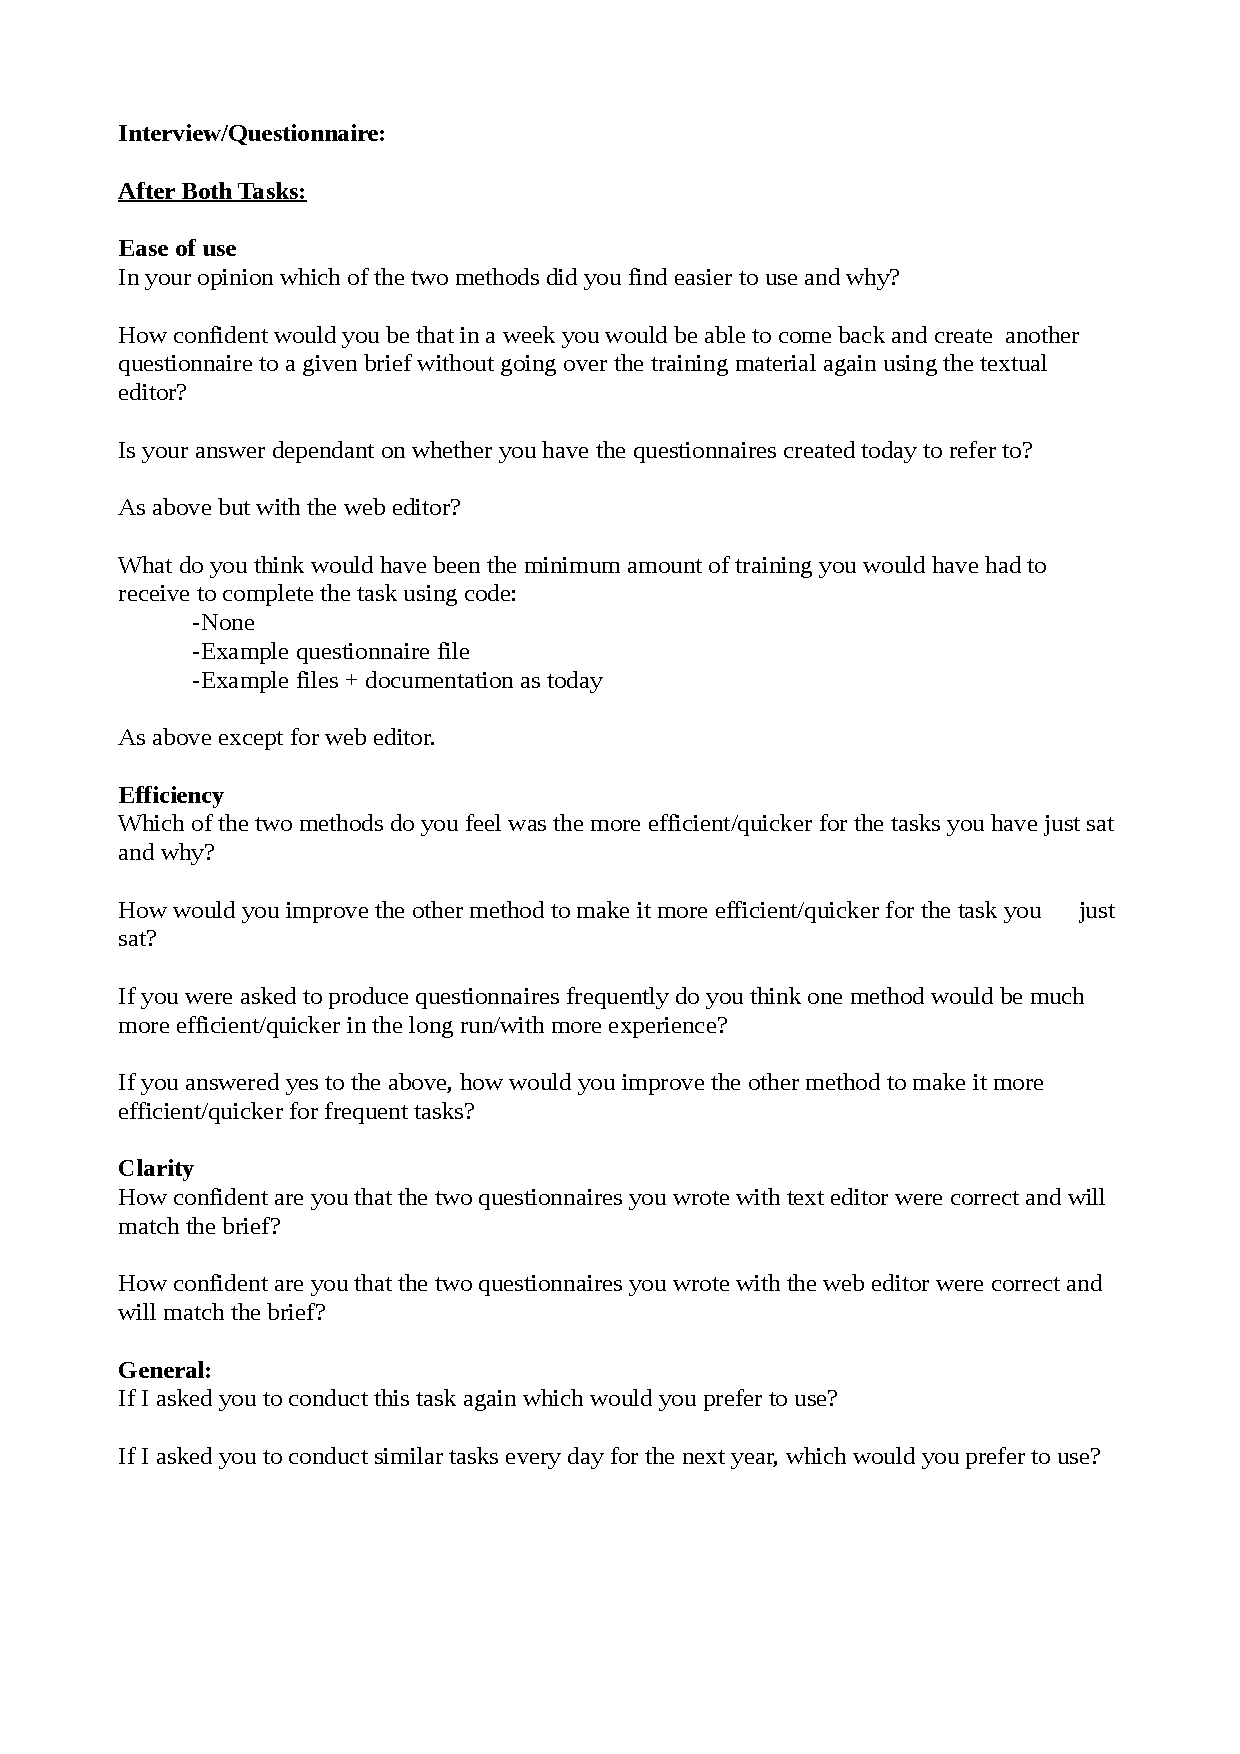
\includepdf[pages=-,scale=.8,pagecommand=\subsection{Interview Questions}]{./Appendix/InterviewQuestions.pdf}

\section{Questionnaire Evaluation Results}\label{questionnaireEvalResults}

\subsection{Respondent 1}
\subsubsection*{First editor used to complete tasks:} Eclipse
\subsubsection*{Times:}
\begin{itemize}
\item \emph{Eclipse Task 1:} 7:28
\item \emph{Eclipse Task 2:} 19:36
\item \emph{Web Task 1:} 2:35
\item \emph{Web Task 2:} 10:25
\end{itemize}
\subsubsection*{Observations made as completing tasks:}

\emph{Eclipse:}
\begin{itemize}
\item Significant confusion caused by curly brace positioning
\item Worried about spacing and initially spent a lot of time trying to perfectly match spaces in example/ training documentation
\item Missed string quotation marks
\item Found the error reporting in Eclipse difficult to deal with, despite positioning of red lines struggled to find where actual error was
\item Confusion from poorly named sections
\item Didn't make use of copy/paste in Android/iPhone section of 2nd task
\item Required help to finish task 2, couldn't work out brace positioning
\end{itemize}
\emph{Web Editor:}
\begin{itemize}
\item Didn't find adding extra sections intuitive, didn't understand how to find section editor and had to ask for help
\item Tried to click on reference to section in main questionnaire view as if it were a link
\item Tried adding goto's to sections that didn't yet exist
\end{itemize}

\subsubsection*{Post Tasks Interview Transcript:}
\textit{In your opinion which of the two methods was the easier to use with the training that you had and why was that? } \\
\\
Definitely the second one
\\
\\
\textit{The web editor?}
\\
\\
Yep.Because having dropdowns made [input easier], you just had to recognise what section to put in as opposed to having to memorise exactly what to type so you just have to be familiar with it as opposed to knowing exactly what to enter. Also not having to put in the brackets in the right places was a massive help.
\\
\\
\textit{If I were to ask you to come again in a weeks time and I were to ask you to create another questionnaire to a given brief but didn't give you the training materials, how confident would you be creating that firstly with the textual editor?}
\\
\\
I'm not even sure I'd be able to create it now, without any errors.
\\
\\
\textit{Would your answer change if you had your previous questionnaires to refer back to so you could see how you'd done things before}\\
\\
No, because even with the training materials today the chances of getting an error were relatively high and the error messages given on the screen weren't terribly intuitive I felt.
\\
\\
\textit{And with the second method [web editor], the same question. If you were to come back in a week and I gave you a questionnaire specification without the training materials, do you think you'd be able to create it from scratch?}
\\
\\
Probably. Yes. I think so yes, it might be a bit slower, but yeh I think I could do it again.
\\
\\
\textit{would you need these examples that you've just created to refer to?}
\\
\\
Probably not, no.
\\
\\
\textit{Efficiency is the next thing we'll talk about. Which of the two methods did you think was quicker?}
\\
\\
The second one. [Web editor] 
\\
\\
\textit{Why did you think that?}
\\
\\
There was less thinking time for me as all the text you have to input wasn't at the front of my brain and so it was a slower process to recall it as I wasn't familiar with it and so that was a bit of a slower process whereas the [web editor] you just had to recognise it so it's much quicker. Also selecting from a drop down is inherently quicker.
\\
\\
\textit{If I were to force you to use the textual editor, how would you make it quicker for you and more efficient?}
\\
\\
Get rid of all the brackets
\\
\\
\textit{So actually changing the language itself?}
\\
\\
Yes, or introduce software that puts them in automatically. As with the Answers surely it's the case that they always have to have those so you could automatically install those. Or have clearer error messages saying where you have to put one.
\\
\\
\textit{If you were to produce these questionnaires really frequently, and you had much more experience with both methods, do you think that would change your answer? Do you think you would still be quicker with the web editor or do you think you would get used to the language to a point where you'd be quicker with that?}
\\
\\
No I think it'd still be quicker with the web editor, but obviously you'd get quicker with the text editor too I think I'd still be faster with the web editor.
\\
\\
\textit{How confident were you that the questionnaires you wrote with the text editor matched the specification?}
\\
\\
Well, apart from the errors which meant it wouldn't have run at all, once those had been corrected I guess relatively confident. I don't know, I've never seen one of these run so I don't know.
\\
\\
\textit{And what about with the web editor?}
\\
\\
Well, because I selected everything from dropdowns in the editor I assume that selecting those options would produce like the website correctly.
\\
\\
\textit{Sorry, I'm asking here not whether or not it'd be able to do the conversion, but whether you think the specification that you typed matches the one given. Does that make sense?}
\\
\\
Yep. Relatively confident, I think. It was quite clear by going back to the questionnaire which sections you had, which I think helps.
\\
\\
\textit{So in general if I were to ask you to do this task again which would you use?}
\\
\\
The web editor.
\\
\\
\textit{And if I were to ask you to do it every day for a year, does that change your opinion?}
\\
\\
I do wonder if selecting drop downs might be more boring, but it is more efficient. But then if this were my job I'd probably be bored either way, so web editor.
\subsection{Respondent 2}
\subsubsection*{First editor used to complete tasks:} Eclipse
\subsubsection*{Times:}
\begin{itemize}
\item \emph{Eclipse Task 1:} 4:24
\item \emph{Eclipse Task 2:} 17:05
\item \emph{Web Task 1:} 3:30
\item \emph{Web Task 2:} 11:03
\end{itemize}
\subsubsection*{Observations made as completing tasks:}

\emph{Eclipse:}
\begin{itemize}
\item Spent significant time during training looking at example file
\item Made use of copy and paste functionality to take structure from example file and modify the relevant fields
\item Unsure about spacing and asked several times if mattered
\item Struggled with curly braces
\item Made use of copy and paste within second task on Android/iPhone sections
\item Missed a curly brace. Despite error underlining where it should be added and error message "Missing '\{'' " respondent assumed issue was elsewhere in the file and to do with spacing. Took sometime to spot real cause
\end{itemize}
\emph{Web Editor:}
\begin{itemize}
\item Found confusing had to add section before could cross reference
\item Did use the sub tree views to modify just a particular question
\end{itemize}

\subsubsection*{Post Tasks Interview Transcript:}

\textit{First question is which of the two methods did you find easier to use and why?}
\\
\\
In terms of actual use in terms of which was more intuitive to work out, the web based one. The web based editor. Although as I got more used to the eclipse editor that became easier and quicker to use because when the surveys got more repetitive it was easier to just copy and paste and also to change things retrospectively.
\\
\\
\textit{If I were to ask you to come back in a week and write another questionnaire, how confident would you be that you'd be able to do that? Firstly in the web editor, without the training materials.}
\\
\\
Far easier than the text editor. As said it was far more intuitive
\\
\\
\textit{And what about with the eclipse editor?}
\\
\\
I think with the eclipse, perhaps if I had the example coding but writing it completely from scratch would be a lot more difficult.
\\
\\
\textit{So you think if you had the example code you would be able to do that, using one of the files you wrote today say to refamiliarise yourself?}
\\
\\
If all the necesary sections were there, then yes. If there were other things that I hadn't been taught then the web based editor would be easier.
\\
\\
\textit{And with the textual, Eclipse editor what do you think the minimal amount of training you would have had to receive? If I'd have sent you an exisiting questionnaire and then a task do you think you could have worked out how to write a specification from the example?}
\\
\\
I believe so yes,but I think if it's the kind of thing you'd keep coming back and forth from, it'd still take a lit of time to relearn it unless you were consistently coding.
\\
\\
\textit{And what about the web editor, do you think you could have used that without any of the documentation you received today?}
\\
\\
Yes I think so, at least with the example questionnaire to map it. Particularly if it was something you could map in advance as you add sections in order so as long as you'd planned it in advance and you had an idea of what your questionnaire would look like it's much easier to map and then once that's in place it's not that bad to intuitively put things together.
\\
\\
\textit{I'm now going to ask you some questions about the efficiency of the two methods. Firstly, which of the two methods do you think was quicker/more efficient, using the terms interchangeably here. For the task that you've just sat, and why?}                                                                                                                                                                                                                                                                \\
\\
I think initially the web based editor was more efficient, but once you'd got to grips with what Eclipse was asking for that became quicker as the tasks progressed. I certainly found answering task 1 easier on the web page than task 1 on Eclipse. But then once you'd kind of got used to it, especially with example code to copy and paste I found that was more efficient.
\\
\\
\textit{How would you improve the web editor then to make it more efficient?}
\\
\\
I think the ability to move sections around and actually be able to edit and duplicate sections. Like the last function on Android or iPhone they are asking for the same thing mapped in the same way and that was easy to copy and paste in the text editor and if you could do that in the web editor that would make things easier. Also if someone were proficient in not necessarily coding but questionnaires or whatever it is they're mapping, if there's not a set plan there should be more room for them to change things as they're doing it. I'm not sure how that manifests itself with this tree, maybe some kind of flowchart where they could move things around. But I think that would make it more intuitive for the purpose of making. Since I think the whole point of this is to make things easier.
\\
\\
\textit{If I were to ask you to produce these questionnaires frequently do you think in the long run one method would be more efficient?}
\\
\\
With more experience I think I'd become more proficient at the code based [eclipse editor] but if you implemented the changes to make the [web based] more free flowing I think that would be easier in the long run. Even if someone is proficient at coding there is still the risk of human error when you're producing stuff with code as opposed to being funnelled through the web page program.
\\
\\
\textit{If I were to give you a questionnaire written by someone else, that had an issue with it, with specification, such as a spelling mistake or being taken to the wrong section. Which of the two methods would yuou prefer to find that mistake?}
\\
\\
I'd say in that case the text based as you can have all the code in front of you and have an open plan of everything I think the web based is more efficient at times since it funnels you into stuff but if theres a clear problem you have to open every step to look for it.
\\
\\
\textit{If we were to change the web based program to display everything and you had the option to narrow down only if you wanted to, would that change your answer?}
\\
\\
Yes if you added a checkbox on the tree to show all to explode the view that would be very useful and would have all the benefits of the text based editor.
\\
\\
\textit{If I were to ask you to create another survey right now, which of the two methods would you use?}
\\
\\
If it was utilising all the same methods as previously done in the first two tasks I would go for the text based because if the code were in front of me I could copy and paste the layout. If there were anything new or new functions I think the web based would be more efficient
\\
\\
\textit{If I were to ask you to create another survey every day for a year, does your answer change?}
\\
\\
Probably wouldn't change, but if you implemented the changes I suggested that would probably be more efficient.
                                                                                                                                                                                                                                                                                                                                                                                                                                                                                                                                                                                                                                                                                                                                                                                                                                                                                                                                                                                                                                                                                                                                                                                                                                                                                                                                                                                                                                                                                                                                                                                                                                                                                                                                                                                                                                                                                                                                                                                                                                                                                                                                                                                                                                                                                                                                                                                                                                                                                                                                                                                                                                                                                                                                                                                                                                                                                                                                                                                                                                                                                                                                                                                                                                                                                                                                                                                                                                                                                                                                                                                                                                                                                                                                                                                                                                                                                                                                                                                                                                                                                                                                                                                                                                                                                                                                                                                                                                                                                                                                                                                                                                                                                                                                                                                                                                                                          

\subsection{Respondent 3}
\subsubsection*{First editor used to complete tasks:} Web
\subsubsection*{Times:}
\begin{itemize}
\item \emph{Eclipse Task 1:} 4:03
\item \emph{Eclipse Task 2:} 15:14
\item \emph{Web Task 1:} 3:19
\item \emph{Web Task 2:} 10:57
\end{itemize}
\subsubsection*{Observations made as completing tasks:}

\emph{Eclipse:}
\begin{itemize}
\item Missed 'Section' keyword when creating first section in task 1 and had some difficulty in realising this was the cause of an error as the produced error message wasn't clear. Saying only "EOF was expected"
\item Made use of copy and paste on individual questions, modifying relevant attributes only
\item Had little issue with curly braces, perhaps as made use of Eclipse's automatic insertion of these
\end{itemize}
\emph{Web Editor:}
\begin{itemize}
\item Struggled with navigating between questionnaire editor and section editor at first
\item Confusion caused by adding nodes which are generated from the parse tree but in themselves are meaningless, normally only used for other nodes to inherit
\item Tried clicking on references in questionnaire editor
\item Tried adding references in goto feature despite references not yet existing.
\end{itemize}

\subsubsection*{Post Tasks Interview Transcript:}
\textit{Which of the two methods did you find the easier to use?}
\\
\\
The web editor
\\
\\
\textit{And why was that?}
\\
\\
Found it easier to organise and picture what I was doing with graphics rather than text
\\
\\
\textit{If I were to ask you to come back in a week and write a 3rd questionnaire how confident would you be that you'd be able to code that up with Eclipse, without the training materials?}
\\
\\
Without instructions I wouldn't be that confident.
\\
\\
\textit{Would your answer change if you had the ones today to look back on?}
\\
\\
Yeh if I had the ones from today I could do it again.\\
\\
\textit{What about with the web editor?}
\\
\\
I think I could do it.
\\
\\
\textit{Without any example files?}
\\
\\
Yeh
\\
\\
\textit{What is the minimum amount of training you think you'd need to be able to use these editors? Firstly with the Eclipse editor, do you think you could have completed the tasks using just an example file or even nothing at all?}
\\
\\
No, I don't think I would have been able to I needed the instructions.
\\
\\
\textit{What about with the web editor?}
\\
\\
Yeh I probably would have been able to work it out, maybe with a bit of trial and error.
\\
\\
\textit{Which of the two methods did you think was the more efficient, by which I mean quicker?}
\\
\\
I think the web editor was, it's difficult because once I'd already created the survey once it made it easier the second time around but I thought that the web editor was quicker.
\\
\\
\textit{How would you make the Eclipse editor to make it more efficient for the tasks you've just done? Do you think it was missing anything that would have made it easier?}
\\
\\
I just found it slightly difficult to keep track of where the different sections I had created and in visualising it. But I'm not sure how you could improve it from that.
\\
\\
\textit{If I were to ask you to create these questionnaires frequently do you think your answer as to which was more efficient would change given more experience?}
\\
\\
No, there's not really any benefit from the text editor that I'd get having used it more. I don't know, I don't think they'd change much.
\\
\\
\textit{Is there anyway you could improve it either method to make them more efficient in the long run}
\\
\\
I can't think of anything.
\\
\\
\textit{The company you work for come back to you with a questionnaire and they said that there is an issue with it. Something like the sections are out of order or a spelling mistake was present. Which editor do you think would make it easier to find the mistake?}
\\
\\
I suppose the web editor, there's less going on. It'd probably be quite close as the text editor [Eclipse] did give some warnings that pop up. But you have fewer things on your screen with the web editor.
\\
\\
\textit{If I were to ask you to do this task again which would you prefer to use?}
\\
\\
The web editor
\\
\\
\textit{And if I were to ask you to do this again every day for a year which would you prefer to use?}
\\
\\
Web editor


\subsection{Respondent 4}
\subsubsection*{First editor used to complete tasks:} Web
\subsubsection*{Times:}
\begin{itemize}
\item \emph{Eclipse Task 1:} 5:58
\item \emph{Eclipse Task 2:} 17:54
\item \emph{Web Task 1:} 4:43
\item \emph{Web Task 2:} 11:04
\end{itemize}
\subsubsection*{Observations made as completing tasks:}

\emph{Eclipse:}
\begin{itemize}
\item Had to be shown where the curly braces were on a keyboard
\item Didn't use curly braces at one point with a multiple choice question, read error "Need \{ at Answer" which ellicited a "What?" response. Had to spend some time comparing with example file before understood.
\item Surprised by the automatic insertion of "\}" which caused some initial confusion
\item Missed quotation marks around strings in titles and questions to begin with, visibly frustrated by the error which appeared. "What's wrong now!"
\item Was worried about spacing and tried to copy that of example exactly initially 
\end{itemize}
\emph{Web Editor:}
\begin{itemize}
\item Struggled to navigate tree to find the section editor, during both tasks. 
\item First attempted to add section references in goto before they had been added. Once discovered couldn't do this left all goto statements to fill in at end of the task
\item When filling in goto's at end of task found it very difficult to navigate to individual sections as name wasn't in tree
\end{itemize}

\subsubsection*{Post Tasks Interview Transcript:}
\textit{In your opinion which of the two methods was easier to use?}
\\
\\
The first one
\\
\\
\textit{The web editor?}
\\
\\
Yes
\\
\\
\textit{Why was that?}
\\
\\
it was more intuitive and involved less typing
\\
\\
\textit{What was it about the typing that you found difficult then?}
\\
\\
So not necessarily the typing but remembering which extra symbols I needed to include and at which points like the brackets and the quotation marks.
\\
\\
\textit{If I were to come back in a week to create another questionnaire to a different specification, how confident would you be that you'd be able to create that questionnaire using the text editor without the training materials?}
\\
\\
Not at all, I'll have forgotten this by tomorrow.
\\
\\
\textit{What about if you had an example to refer to?}
\\
\\
I think if I had the tasks I just did now to refer to I'd be able to pick it up again, but it would be harder.
\\
\\
\textit{What about with the web based editor?}
\\
\\
That would be easier I don't even think I'd need anything to refer to.
\\
\\
\textit{With the text editor, today you had some documentation and an example file. Do you think you could have done the tasks without either of those things?}
\\
\\
No
\\
\\
\textit{You needed both?}
\\
\\
I needed both, I used both.
\\
\\
\textit{What about with the web editor, could you have done the task without the documentation?}
\\
\\
It was helpful to look at it, but I don't think I would need to look at it again.
\\
\\
\textit{Which of the two methods did you think was the most efficient or quicker?}
\\
\\
The web editor
\\
\\
\textit{And why did you think that?}
\\
\\
Just objectively I think it took less time
\\
\\
\textit{And how would you improve the text editor to make it more efficient?}
\\
\\
I don't know, I don't think you could improve the text editor yourself, you'd just have to get better at it. I mean, if you were to do this everyday you'd get better at it.
\\
\\
\textit{That's actually the next question, so if you were to do these questionnaires frequently do you think one method would be more efficient then?}
\\
\\
So I think you could get as good with the text editor as with the web one but I don't know that, in the long term, one would be more efficent.
\\
\\
\textit{Say I were your boss and I were to come to you with a questionnaire that Jeff wrote and said it had a mistake in it. This mistake definitely lies with the way it's been specified so is either a spelling mistake or sections are in the wrong order. Which method would be easier to find the mistake?}
\\
\\
Web editor.
\\
\\
\textit{And why is that?}
\\
\\
Because with the text editor you'd have to go through the entire text whereas with the web editor you can go into the individual sections and find it more easily.
\\
\\
\textit{And what if you didn't know which section it was in? Say the questionnaire has ten sections in it and a question leads you to the wrong section.}
\\
\\
The text editor then. Actually I don't know, I think it would depend.
\\
\\
\textit{If I were to ask you to create a third survey now which method would you use?}
\\
\\
The web editor
\\
\\
\textit{And if I were to ask you to create one every day for a year which would you use?}
\\
\\
The web editor
\subsection{Respondent 5}
\subsubsection*{First editor used to complete tasks:} Eclipse
\subsubsection*{Times:}
\begin{itemize}
\item \emph{Eclipse Task 1:} 11:01
\item \emph{Eclipse Task 2:} 18:25
\item \emph{Web Task 1:} 3:19
\item \emph{Web Task 2:} 11:42
\end{itemize}
\subsubsection*{Observations made as completing tasks:}

\emph{Eclipse:}
\begin{itemize}
\item Had to be shown where the curly braces were on a keyboard
\item Unsure about spacing in layout of file
\item spaces added to MultipleChoiceQuestion keyword
\item Used example to refer to alot
\item Caught out on one occasion by automatic addition of closing brace by IDE. Found this easily later though
\item Struggled with referencing in the second task alot, added goto reference for section which didn't exist and then as marked as error changed name multiople times, trying to add spacing, quotation marks etc. Until finally realised had to add the section
\end{itemize}
\emph{Web Editor:}
\begin{itemize}
\item Struggled to navigate tree to find the section editor to begin with, although fine after first task
\item Attempted to add section references in goto before they had been added. Once discovered couldn't do this left all goto statements to fill in at end of the task
\end{itemize}

\subsubsection*{Post Tasks Interview Transcript:}
\textit{Which of the two methods was easier to use?}
\\
\\
The second one, the web editor
\\
\\
\textit{And why was that?}
\\
\\
I think having the different options available so you can see how it works and you're less likely to make mistakes in that way as there's a limited amount that can go wrong
\\
\\
\textit{How confident would you be that in a week if I were to ask you to create a questionnaire using the text editor that you'd be able to do it without the training again?}
\\
\\
I probably would be ok, am I allowed the examples?
\\
\\
\textit{Yes}
\\
\\
Then yes probably
\\
\\
\textit{And what if you weren't allowed the examples?}
\\
\\
I think it would take a lot longer, I think I'd get it right eventually but it'd take a while.
\\
\\
\textit{So you think you'd remember how to do it?}
\\
\\
Yes
\\
\\
\textit{What about with the web editor?}
\\
\\
Yes the same I think
\\
\\
\textit{So you think that would be quicker with these [the tasks completed today] to refer to? }
\\
\\
Yes
\\
\\
\textit{With the text editor, what do you think was the minimum amount of training you'd have needed?  Do you think you could have done it without the documentation or without the example file or even without both?}
\\
\\
I think I'd need both
\\
\\
\textit{And with the web editor, do you think you could have done that without documentation?}
\\
\\
No
\\
\\
\textit{Which one did you think was more efficient?}
\\
\\
The web based one
\\
\\
\textit{And why do you think that was the case?}
\\
\\
Maybe because I'd done the other one first which was probably useful. Also the drop down menus meant I didn't have to type everything.
\\
\\
\textit{So how would you improve the textual editor to make it more efficient?}
\\
\\
I don't know. I don't think you could
\\
\\
\textit{If I were to ask you to write these frequently do you think one method would be much better with more experience?}
\\
\\
Yes
\\
\\
\textit{Which one?}
\\
\\
The web based one
\\
\\
\textit{And how would you then improve the textual one to make it more efficient}
\\
\\
I think I'd just have to get more familiar with it. I didn't really know that the crosses meant when something had gone wrong.
\\
\\
\textit{But even with that experience you don't think it would be faster than the web based one?}
\\
\\
No
\\
\\
\textit{If I were to ask you to do the task again now, which would you prefer to use?}
\\
\\
The web editor
\\
\\
\textit{And if I were to ask you to do the same task everyday for a year, which method would you choose if you had to commit to one?}
\\
\\
The web editor

\end{document}